%%%%%%%%%%%%%%%%%%%%%%%%%%%%%%%%%%%%%%%%%%%%%%%%%%%%%%%%%%%%%%%%%%%
\section{Hiérarchie mémoire} \label{sec:hierarchie}
%%%%%%%%%%%%%%%%%%%%%%%%%%%%%%%%%%%%%%%%%%%%%%%%%%%%%%%%%%%%%%%%%%%

\begin{fancyquotes}
Idéalement, on souhaiterait disposer d'une capacité de mémoire indéfiniment grande, de sorte qu'un agrégat particulier de 40 chiffres binaires, ou mot (cf. 2.3), soit immédiatement disponible, c'est-à-dire dans un temps légèrement ou considérablement plus court que le temps de fonctionnement d'un multiplicateur électronique rapide. On peut supposer que cela est pratique au niveau d'environ 100 m sec. Par conséquent, le temps de disponibilité d'un mot dans la mémoire doit être de 5 à 50 ms. Il est également souhaitable que les mots puissent être remplacés par de nouveaux mots à peu près au même rythme. Il ne semble pas physiquement possible d'atteindre une telle capacité. Nous sommes donc obligés de reconnaître la possibilité de construire une hiérarchie de mémoires, chacune d'entre elles ayant une plus grande capacité que la précédente mais moins rapidement accessible.\\
Traduit de \cite{burks1946preliminary}.

\end{fancyquotes}


\subsection{Motivations}
%%%%%%%%%%%%%%%%%%%%%%%%%%%%%%%%%%%%%%%%%%%%%%%%%%%%%%%%%%%%%%%%%%%


Dès 1946, les architectes des processeurs avaient anticipé que les applications seraient demandeuses de mémoires très performantes. A cause de la forte évolution du processeur, l'écart avec la performance des mémoires s'est creusé au fil des années (voir \autoref{pic:cpuvsmemory}). L'incapacité du processeur d'accéder suffisamment rapidement à la mémoire est inhérent à l'architecture actuelle des processeurs qui partage le même bus pour accéder aux instructions et aux données stockées en mémoire. Ce \textit{goulot d'étranglement} ou \textit{bottleneck}, a été nommé d'après l'un des architectes de l'architecture: le \textit{bottleneck Von Neumann}.


\begin{figure}
    \center
    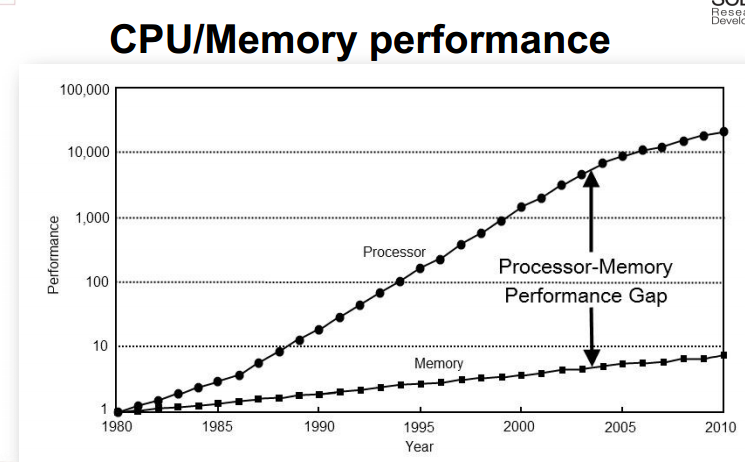
\includegraphics[width=10cm]{images/cpu_vs_memory.png}
    \caption{\label{pic:cpuvsmemory} Progression de la performance des processeurs et des mémoires. Les processeurs ont vu leur performance évoluer de 50\% chaque année, contre 7\% pour les mémoires. L'écart de performance entre les deux matériels s'est creusé de 50\%  chaque année depuis les années 2000 (graphique extrait de \cite{AliSalehi2012}).}
\end{figure}

La réponse naïve à ce problème est de construire de grande mémoire à partir de SRAM, très performante et qui consomme peu d'énergie. Cependant, des contraintes économiques et technique sont à prendre en compte et rendent impossible cette solution. La mémoire SRAM est très cher à produire et nécessite l'utilisation de six transistors pour fonctionner, empêchant la construction de modules denses. Les constructeurs de processeurs ont dû élaborer une solution en prenant en compte la vitesse, la densité et le coût de chacune des technologies mémoires. Au plus une mémoire est rapide, au plus sont coût est élevé. Au plus la densité est élevée, plus le prix par bit stocké est réduit. Au plus la densité est élevé, au plus le temps d'accès est élevé. 






\subsection{Hiérarchie mémoire sur les processeurs récents}
%%%%%%%%%%%%%%%%%%%%%%%%%%%%%%%%%%%%%%%%%%%%%%%%%%%%%%%%%%%%%%%%%%%

La hiérarchie mémoire est la réponse économique et technique apportée aux contraintes évoquées ci dessus. Elle consiste en l'utilisation de différents modules mémoires de tailles, de technologies et de performances différentes. Son objectif peut être résumé à trois points: réduire le coût par bit stocké, augmenter la capacité de la mémoire la plus rapide, améliorer le temps d'accès aux données. La solution est de placer au plus proche du processeur des mémoires très rapide pouvant répondre instantanément aux accès mémoire. Au plus on s'éloigne des unités de calcul, au plus la latence d'accès aux modules mémoires augmente, mais au plus leur prix diminue rendant possible l'utilisation de module de plus grande capacité.


Les différents niveaux de mémoire peuvent être imbriqués, une donnée qui se trouve dans le premier niveau sera aussi stockée dans les modules de niveaux supérieurs.

Lorsque le processeur souhaite accéder à une donnée, il vérifie qu'elle se trouve dans son premier niveau de mémoire et, si ce n'est pas le cas, remonte la hiérarchie jusqu'à la trouver. La performance des applications varie fortement si les données nécessaires sont présentes ou non dans les mémoires proches du processeur. Les programmes doivent essayer de profiter du concept de localité présenté dans la section \autoref{sec:localite}.
\begin{figure}
    \center
    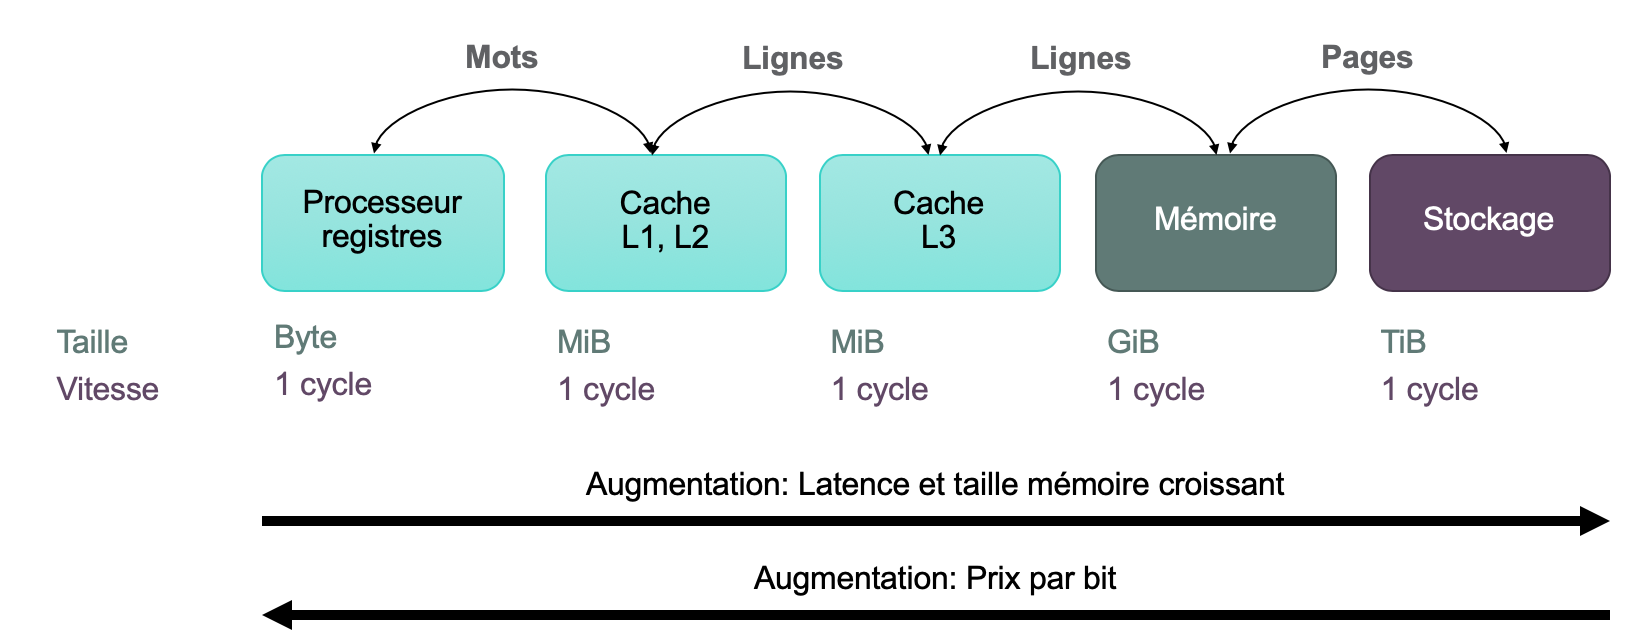
\includegraphics[width=14cm]{images/memory_hierarchy.png}
    \caption{\label{pic:cpuvsmemory} Hiérarchie mémoire}
\end{figure}





\subsection{Communication entre les différents niveaux}
%%%%%%%%%%%%%%%%%%%%%%%%%%%%%%%%%%%%%%%%%%%%%%%%%%%%%%%%%%%%%%%%%%%
Pour communiquer entre les différents niveaux de la hierarchie les données sont transmises par bloc de données de tailles différentes. L'avantage de tranférer les données par bloc et non une par une est d'amlélirer la performance des codes en tirant parti du principe de localité spatiale (voir \autoref{sec:localite}).
Pour accéder à un mot, le processeur a besoin que celle ci se trouve dans le niveau de cache L1. Lorsqu'elle si trouve, le processeur peut charger un mot directement dans ces registres pour y effectuer les opérations nécessaires. C'est la granularité de transfert la plus petite dans un ordinateur. 

Entre les différents niveaux de caches et entre le cache et la mémoire les données sont transférées par blocs appellées \textit{lignes de cache} ou \textit{cache line}. La ligne de cache contient une copie des données de la mémoire, un tag contenant des informations sur l'adresse mémoire du bloc de donnée et un \textit{flag} contenant des informations sur la validité de la ligne (voir \autoref{pic:cacheline}). La taille d'une ligne de cache peut varier d'une architecture à l'autre mais il est courant d'utiliser des tailles de 32, 64 ou 128 bytes. Une ligne de cache d'un processeur Intel récent mesure 64 bytes. Elle contient ainsi entre 8 et 16 éléments en double précision. 

\begin{figure}
    \center
    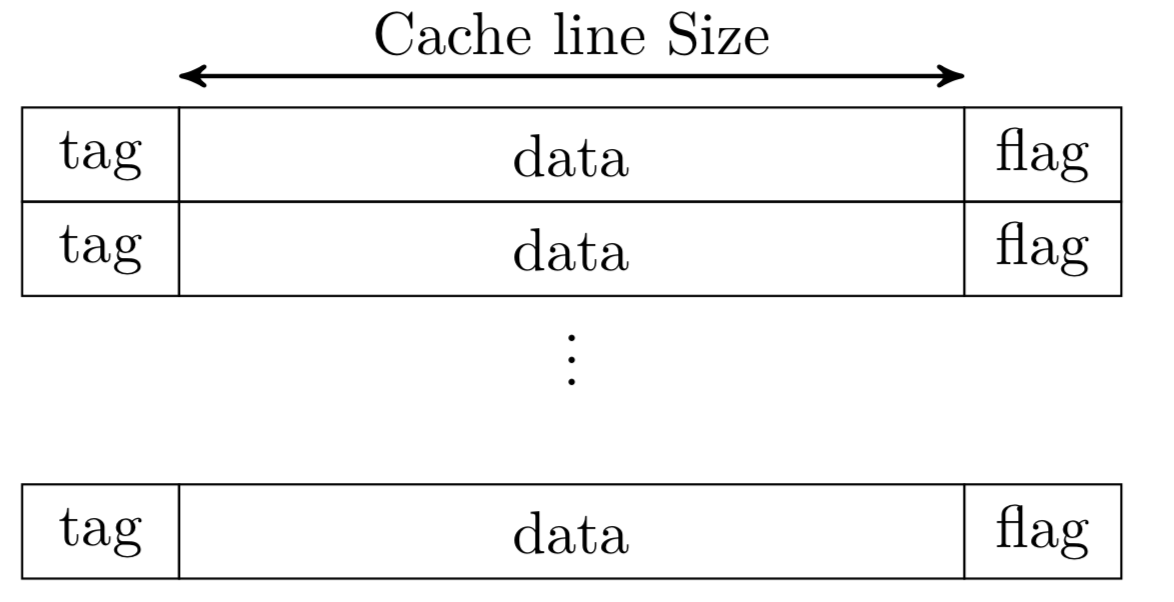
\includegraphics[width=8cm]{images/cacheline_def.png}
    \caption{\label{pic:cacheline} Représentation d'une ligne de cache.}
\end{figure}


Entre la mémoire, les blocs de données transférés sont de la taille d'une page (voir \autoref{sec:page}) qui mesure généralement entre 4 KiB et 2 MiB.



\subsection{Registres}
%%%%%%%%%%%%%%%%%%%%%%%%%%%%%%%%%%%%%%%%%%%%%%%%%%%%%%%%%%%%%%%%%%%
Les registres du processeurs sont situés au plus proche des unités de calculs. Pour permettre un accès rapide, 1 cycle, ils sont réalisés en SRAM. On compte entre x et y registres sur les processeurs récents. Leur taille est variable en fonction des instructions exécutables par les unités logiques arithmétiques. Par exemple, un processeur pouvant exécuter des instructions vectorielles AVX-512, possède des registres de 512 bits (registre \textit{ZMM}). Il existe différents types de registres, certains sont utilisés pour stocker des données et des résultats intermédiaires, tandis que d’autres ont une signification précise. Le registre de pointeurs de piles stocke l’adresse de la première adresse mémoire responsable de l’instruction actuellement exécutée et permettent de réaliser des appels et des retours de fonctions. Les registres des drapeaux (Flag Register) stockent des informations nécessaire à l’éxécution d’instructions. Par exmple, lorsqu’une retenue est générée par un calcul, ou qu’un branchement conditionnelle a été évalué à vrai. Les processeurs récents dupliquent certains registres pour pouvoir utiliser des techniques de renommage \cite{moudgill1993register} et d'exécution spéculative \cite{chou2004efficient}. Lors de l'exécution d'une instruction nécessitant plusieurs cycles, le processeur, si aucune dépendance n'est détectée, commence à exécuter les instructions suivantes sans attendre le résultat de la première instruction.






%%%%%%%%%%%%%%%%%%%%%%%%%%%%%%%%%%%%%%%%%%%%%%%%%%%%%%%%%%%%%%%%%%%
%%%%%%%%%%%%%%%%%%%%%%%%%%%%%%%%%%%%%%%%%%%%%%%%%%%%%%%%%%%%%%%%%%%
\subsection{Caches} \label{sec:cache}
%%%%%%%%%%%%%%%%%%%%%%%%%%%%%%%%%%%%%%%%%%%%%%%%%%%%%%%%%%%%%%%%%%%
%%%%%%%%%%%%%%%%%%%%%%%%%%%%%%%%%%%%%%%%%%%%%%%%%%%%%%%%%%%%%%%%%%%
%intro
C’est en 1965 que les premières mémoires caches sont présentées sous le nom de \textit{slave memory} \cite{wilkes1965slave}. Leur temps d’accès est de 4 à 20 fois plus rapide que celui de la mémoire principale servant alors de mémoire tampon. Cependant leur taille est très réduite (quelques MiB) comparée à celle de la mémoire principale (plusieurs GiB). Les cache utilisent généralement de la mémoire SRAM.

%performance
Ce niveau de mémoire a été implémenté pour réduire, du point de vu du processeur, l’écart de performance entre ses unités de calculs et celles de la mémoire centrale. Leur apport de performance vient de la capacité des programmes à réutiliser des données déjà présentes, évitant une accès à la mémoire centrale beaucoup plus long. Lorsque le processeur doit accéder à une donnée, il commence par la chercher dans le premier niveau de cache, si elle si trouve, son temps d'accés est très rapide (évenement \textit{cache hit}). Si ce n’est pas le cas (évenement \textit{chache miss}), il réalise alors une copie de la zone mémoire la contenant dans le cache. La zone mémoire copié est appelé \textit{ligne de cache}. Si par la suite, cette donnée ou une donnée appartement à la même ligne de cache devait être à nouveau accédée, leur temps d’accès serait alors drastiquement réduit. Ce mécanisme est transparent pour l’utilisateur, bien que pour des questions de performances il doive être conscient de son existence (voir \autoref{sec:localite}). 

%taille vs performance
La taille de chaque niveau de cache varie pour les raisons expliquées en introduction de cette partie. A cela vient s'ajouter la notion de performance qui est liée à leur taille. Un cache de grande capacité aura plus de chance de contenir la donnée dont le processeur à besoin, améliorant ainsi la performance moyenne du programme. Un cache est une mémoire associative. Pour accéder à son contenu il faut utiliser une clef associative. La clef est constitué de l’adresse en mémoire centrale de l’instruction ou de la donnée. Un cache plus grand nécessite plus de comparaisons pour vérifier si une donnée s'y trouve ou non. Pour allier les avantages et contourner les inconvénient, les processeurs utilisent non pas un, mais plusieurs niveaux de caches de tailles différentes.
Le premier niveau de cache est généralement séparé en deux zones mémoire: l'une contenant les instructions et l'autre les données. C'est le seul niveau de la hiérarchie qui stocke différemment les données et les instructions. Sur les processeurs récents, le premier et le deuxième niveau de cache est privé à chaque coeur. Un troisième, et parfois un quatrième niveau de cache est partagé entre les différents coeurs du processeur. La \autoref{pic:cache_hierarchy} représente une telle architecture pour un processeur à 4 coeurs. Le partage d’un ou plusieurs niveaux de caches entre différents coeurs à certains bénéfices en programmation parallèle. La communication entre les coeurs est plus rapide, ainsi que la migration d’un thread entre deux coeurs partageant un même niveau de cache. Cependant, cela introduit de la complexité pour la cohérence des caches (voir \autoref{sec:cache_coherence}).

\begin{figure}
    \center
    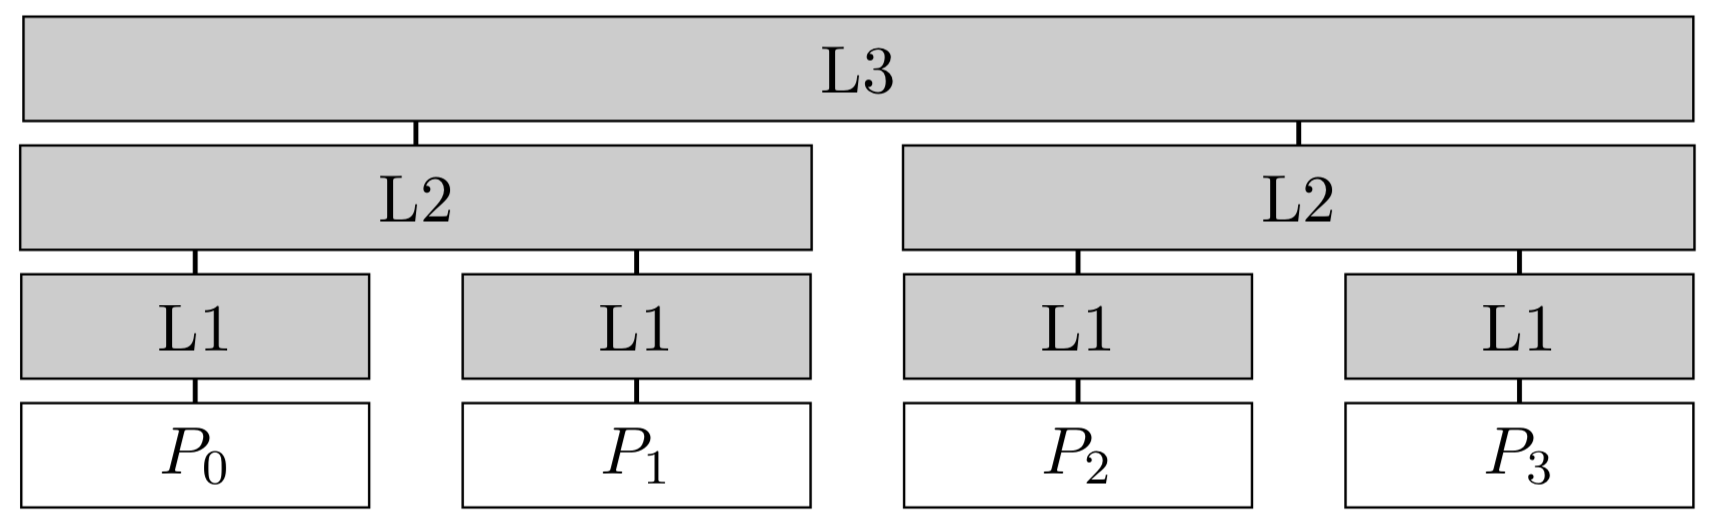
\includegraphics[width=8cm]{images/cache_hierarchy.png}
    \caption{\label{pic:cache_hierarchy} Organisation d'une hiérarchie de cache à trois niveau sur un processeur à 4 coeurs (source \cite{putigny2014benchmark}).}
\end{figure}




\subsubsection{Propriété d'inclusion}
%%%%%%%%%%%%%%%%%%%%%%%%%%%%%%%%%%%%%%%%%%%%%%%%%%%%%%%%%%%%%%%%%%%
Lorsqu'une donnée est chargé depuis la mémoire, le processeur doit la stocker dans le cache qui varie en fonction de la propriété d'inclusion du processeur pouvant être inclusive ou exclusive ou non-inclusive (voir \autoref{pic:cacheinclusionpolicy}).

Un cache est dit inclusif, si lorsqu'une donnée se trouve à un niveau de la hiérarchie, tous les caches des niveaux supérieur contiennent eux aussi une copie de la donnée (voir \autoref{pic:InclusivePolicy}). Cette politique d'inclusion a un désavantage lorsqu'elle est utilisée sur des système multi-coeurs. En effet, lorsqu'une donnée doit être retiré d'un niveau de cache, le processeur doit aussi l'enlever des niveaux de caches inférieurs. 
Un cache non-inclusif permet qu'une ligne du cache de niveau 1 ne soit pas forcément dans le cache de niveau 2. Cela permet d'augmenter la capacité de la hiérarchie de cache. Les processeurs récents implémente les deux politiques d'inclusion. Le processeur Intel Sandy Bridge a un cache L3 inclusif tandis que les cache L1 et L2 sont non-inclusif.

Pour une politique d'exclusion, une donnée qui se trouve à un niveau du cache, ne peut pas se trouver dans un autre niveau de cache au même moment (voir \autoref{fig:ExclusivePolicy}). L'avantage des caches exclusif est leur capacité de stocker plus de données car une ligne de cache ne se trouve jamais à deux endroits à la fois de la hiérarchie de cache. Cependant, lors d'un \textit{hit} dans le cache L2, le processeur doit échanger la ligne entre les deux niveau de cache L1 et L2, plus long qu'une simple copie.



\begin{figure}
    \centering
    \begin{subfigure}[b]{0.45\linewidth}
        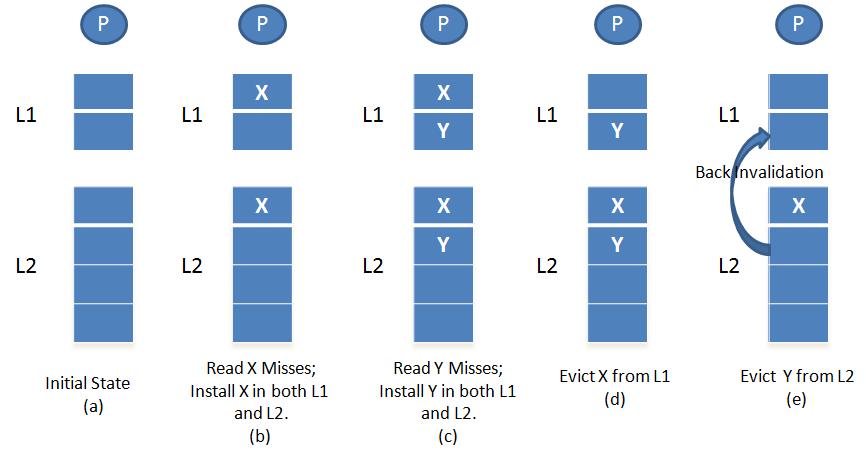
\includegraphics[width=\linewidth]{images/InclusivePolicy.png}
        \caption{Inclusive}
        \label{pic:InclusivePolicy}
    \end{subfigure}
    ~ %add desired spacing between images, e. g. ~, \quad, \qquad, \hfill etc. 
      %(or a blank line to force the subfigure onto a new line)
    \begin{subfigure}[b]{0.45\linewidth}
        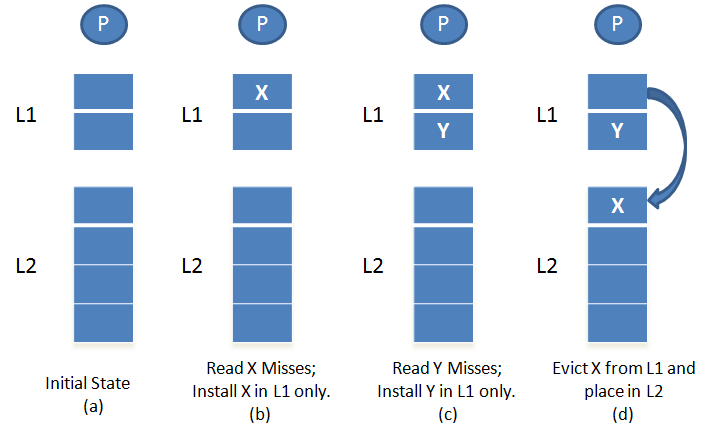
\includegraphics[width=0.85\linewidth]{images/ExclusivePolicy.png}
        \caption{Exclusive}
        \label{pic:ExclusivePolicy}
    \end{subfigure}
    \caption{Exemple de deux propriétés d'inclusion de la hiérarchie de cache (source \cite{wikipedia_2019}). }\label{fig:cacheinclusionpolicy}
\end{figure}




\subsubsection{Politique de placement: associativité}
%%%%%%%%%%%%%%%%%%%%%%%%%%%%%%%%%%%%%%%%%%%%%%%%%%%%%%%%%%%%%%%%%%%
La performance d'un cache ne vient pas seulement de la technologie utilisée pour sa construction. En effet, lorsqu'une donnée est accédée, le cache doit vérifier si la donnée est présente ou non dans le niveau de cache demandé. Il faut que l'algorithme de comparaison permettant de la trouver soit le plus rapide possible. Pour cela, les architectes utilisent généralement une fonction de \textit{hash} permettant d'attribuer un emplacement dans le cache en fonction de l'adresse mémoire de la \textit{cache line}. Si la \textit{cache line} ne se trouve pas à l'emplacement calculé, c'est quelle n'est pas présente dans ce niveau de cache.


\begin{figure}
    \centering
    \begin{subfigure}[b]{0.45\linewidth}
        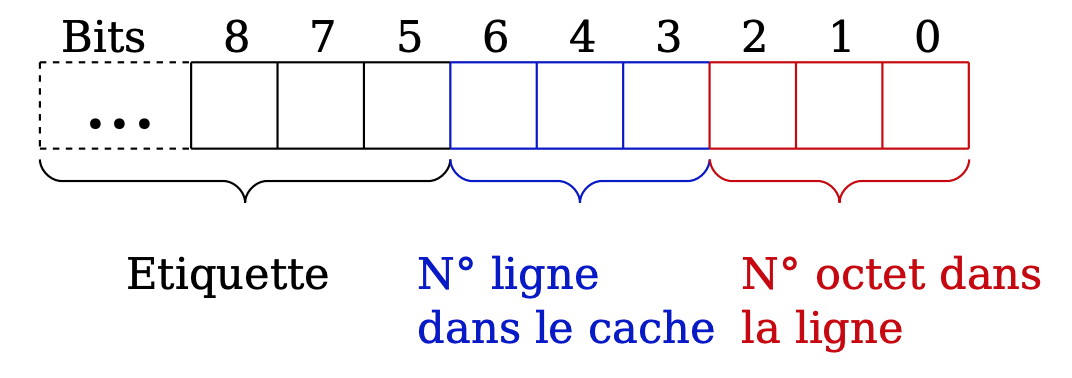
\includegraphics[width=\linewidth]{images/cache_calcul.png}
        \caption{Calcul de l'emplacement (index de la ligne et décalage) pour un mappage direct}
        \label{pic:cache_calcul}
    \end{subfigure}
    ~ %add desired spacing between images, e. g. ~, \quad, \qquad, \hfill etc. 
      %(or a blank line to force the subfigure onto a new line)
    \begin{subfigure}[b]{0.45\linewidth}
        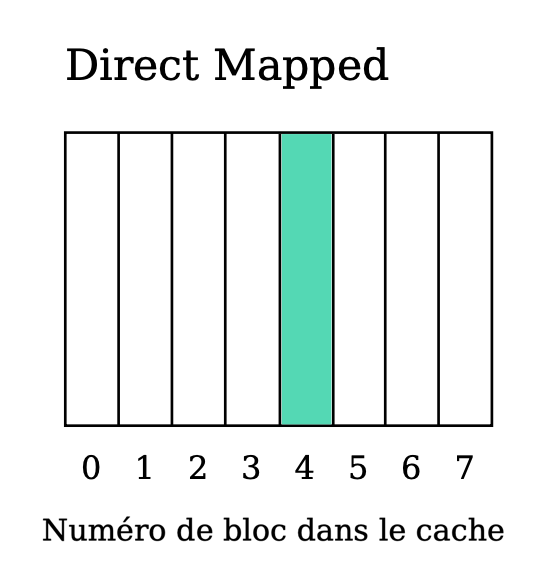
\includegraphics[width=\linewidth]{images/cache_direct.png}
        \caption{Emplacement de la ligne calculée dans le cache ou sera stockée la \textit{cache line}.}
        \label{pic:cache_direct}
    \end{subfigure}
    \caption{Exemple du calcul de l'emplacement de la ligne de cache lors d'un mappage direct à partir de l'adresse de la \textit{cache line} à stocker (source \cite{Meunier2017}). }\label{fig:cacheinclusionpolicy}
\end{figure}





Les trois politiques de placement les plus utilisées sont: le mappage  \textit{direct }, le mappage \textit{fully associative} et le mappage \textit{set assiociative} (voir \autoref{pic:cache_associativite}).


\begin{figure}
    \center
    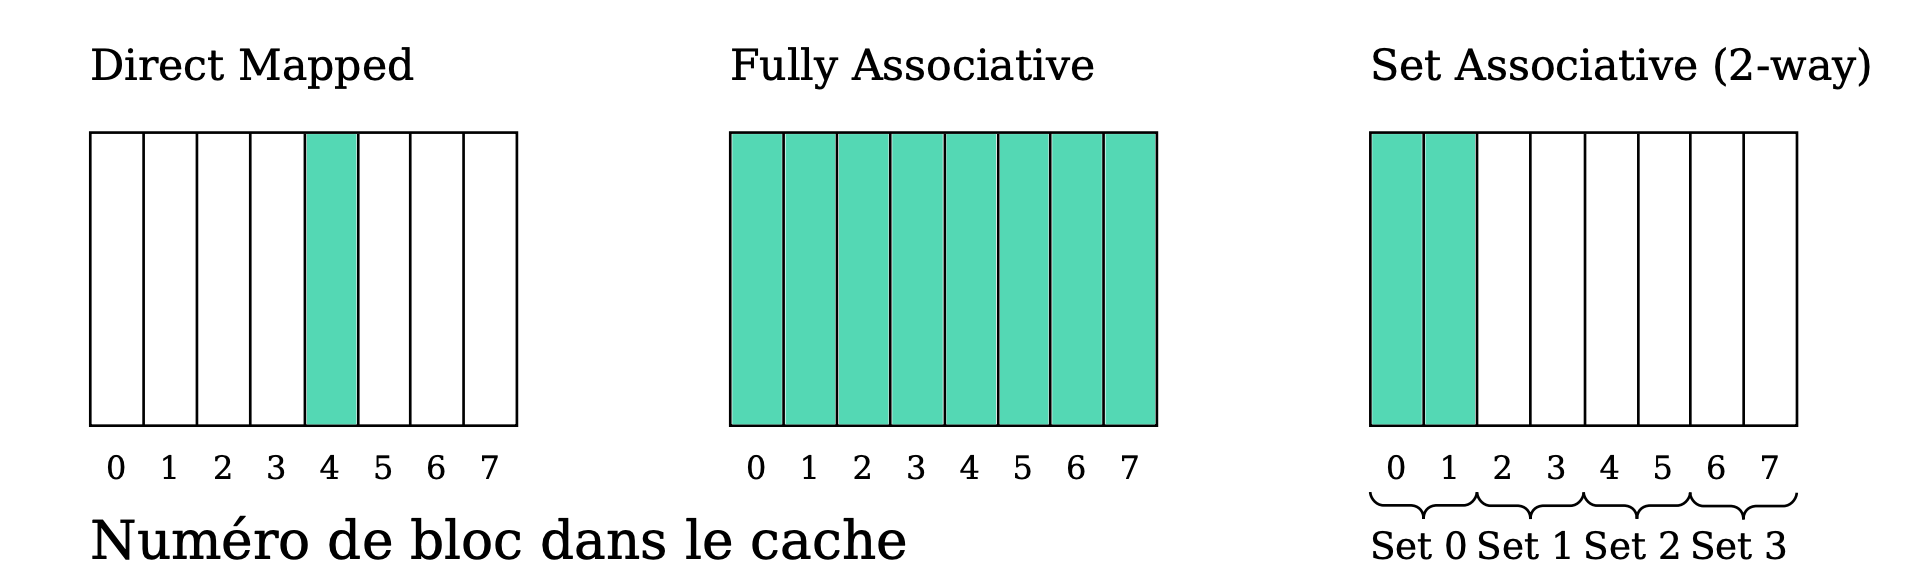
\includegraphics[width=12cm]{images/cache_associativite.png}
    \caption{\label{pic:cache_associativite} En fonction de la politique de remplacement utilisée, une \textit{cache line} sera associée à une ligne du cache différente (source \cite{Meunier2017})}
\end{figure}

\paragraph{Cache à correspondance directe (\textit{direct-mapped cache})} utilise une fonction simple pour déterminer l'emplacement (index et offset) du cache à utiliser. Une partie des bits le l'adresse de la \textit{cache line} est utilisée pour déterminer la ligne à utiliser (\textit{index}) par exemple à l'aide d'une opération modulo. L'autre partie est utilisée pour déterminer le décalage dans cette ligne (\textit{offset}). Cette méthode est très rapide mais peut avoir des performances catastrophiques. Un algorithme faisant des sauts en mémoire d'une certaine taille pourrait n'utiliser qu'une seule ligne du cache, le rendant totalement inefficace. Comparé aux caches associatifs, le mappage direct est plus simple à implémenter car un seul comparateur est nécessaire pour déterminer la ligne de cache à utiliser (voir \autoref{fig:cache_schema}).

\paragraph{Cache pleinement associatif (\textit{fully associative cache})} remédie à ce problème en permettant à une \textit{cache line} d'être stockée à n'importe quel emplacement dans le cache. Cependant, cette technique à le désavantage d'être très lente. En effet, une \textit{cache line} pouvant se trouver à n'importe quelle ligne du cache, il faut toutes les comparer pour vérifier sa présence ou non. Pour faire cette comparaison en parallèle, il faudrait implémenter autant de comparateurs que de ligne dans le cache, complexifiant grandement le cache.


\paragraph{Cache N-associatif (\textit{N-way set associative cache})} permet de réduire le nombre de comparateurs nécessaires en regroupant les lignes du caches potentiellement adressable pour une \textit{cache line} en groupe (\textit{set}). L'exemple de la \autoref{pic:cache_associativite} utilise un cache à 4 set, appelé \textit{4-way associative}. Il ne faut plus que 4 comparateurs pour déterminer si une ligne appartient à un des \textit{set}. Les mappage par association sont plus lents que le mappage direct, car il faut trouver où se trouve la \textit{cache line} (si présente) dans un sous ensemble de ligne de cache plus ou moins grand. Pour accélérer la recherche de la présence ou non d'une ligne de cache, le traitement peut être réalisé en parallèle dans les différents \textit{sets} par l'utilisation de plusieurs comparateurs (4 dans la \autoref{pic:cache_circuit-set-associative}). 

La propriété principale d'un cache est sa capacité à conserver les données pour de futurs accès. Un cache de 8 MB à 2 set associatifs peu sauver jusqu'à 44\% des \textit{miss} comparé à un cache à correspondance directe \cite{Drepper2007}. Sur les architectures récentes Intel Skylake, les caches utilisent entre 8 et 16 associativités, pouvant varier entre les différents niveaux. 

\begin{figure}
    \centering
    \begin{subfigure}[b]{0.45\linewidth}
        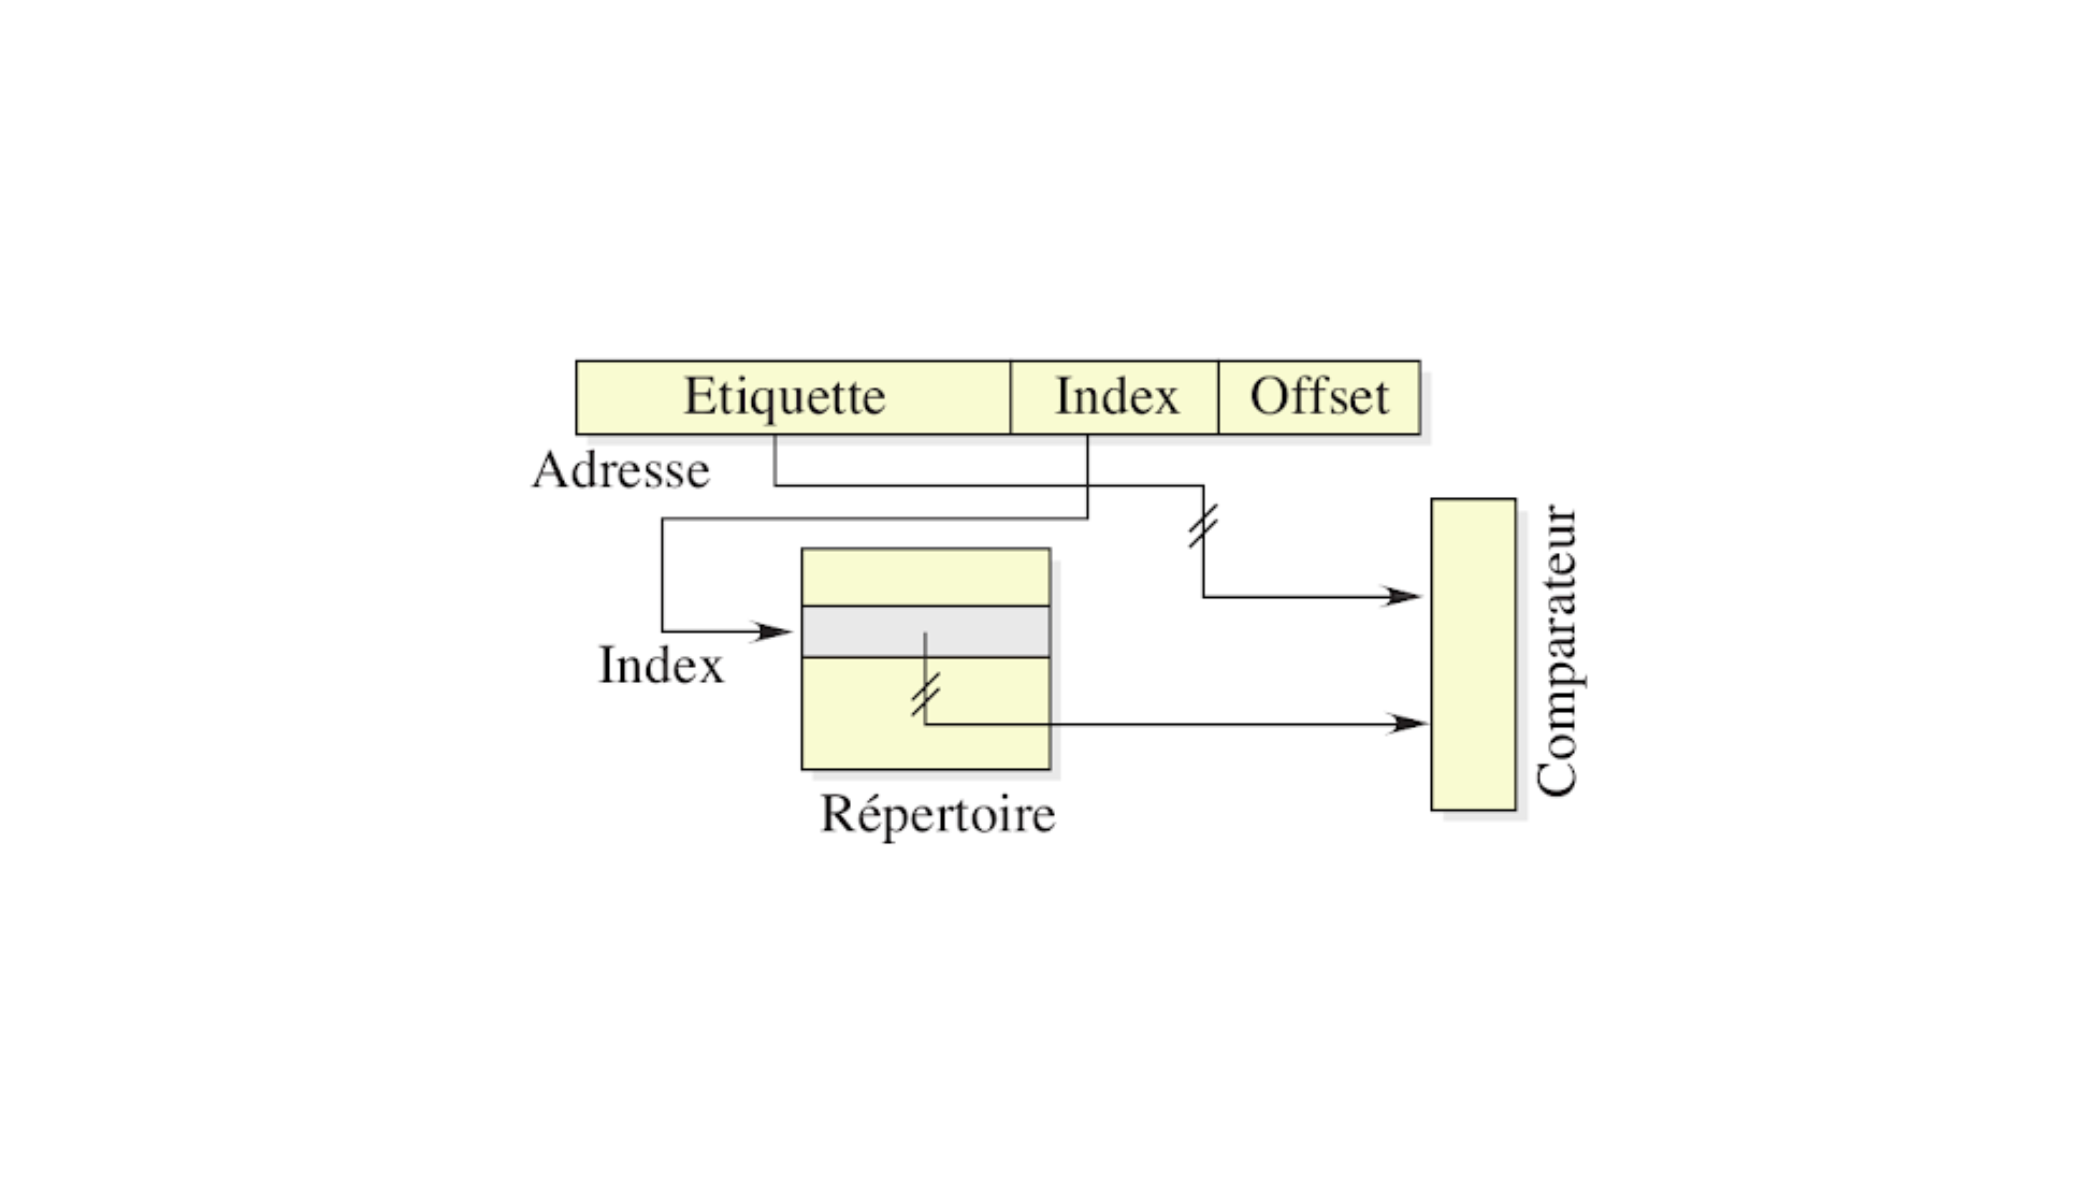
\includegraphics[width=\linewidth]{images/cache_circuit-direct.png}
        \caption{Le cache pleinement associatif nécessite d'avoir un comparateur pour chacune des lignes du cache}
        \label{pic:cache_circuit-direct}
    \end{subfigure}
    ~ %add desired spacing between images, e. g. ~, \quad, \qquad, \hfill etc. 
      %(or a blank line to force the subfigure onto a new line)
    \begin{subfigure}[b]{0.45\linewidth}
        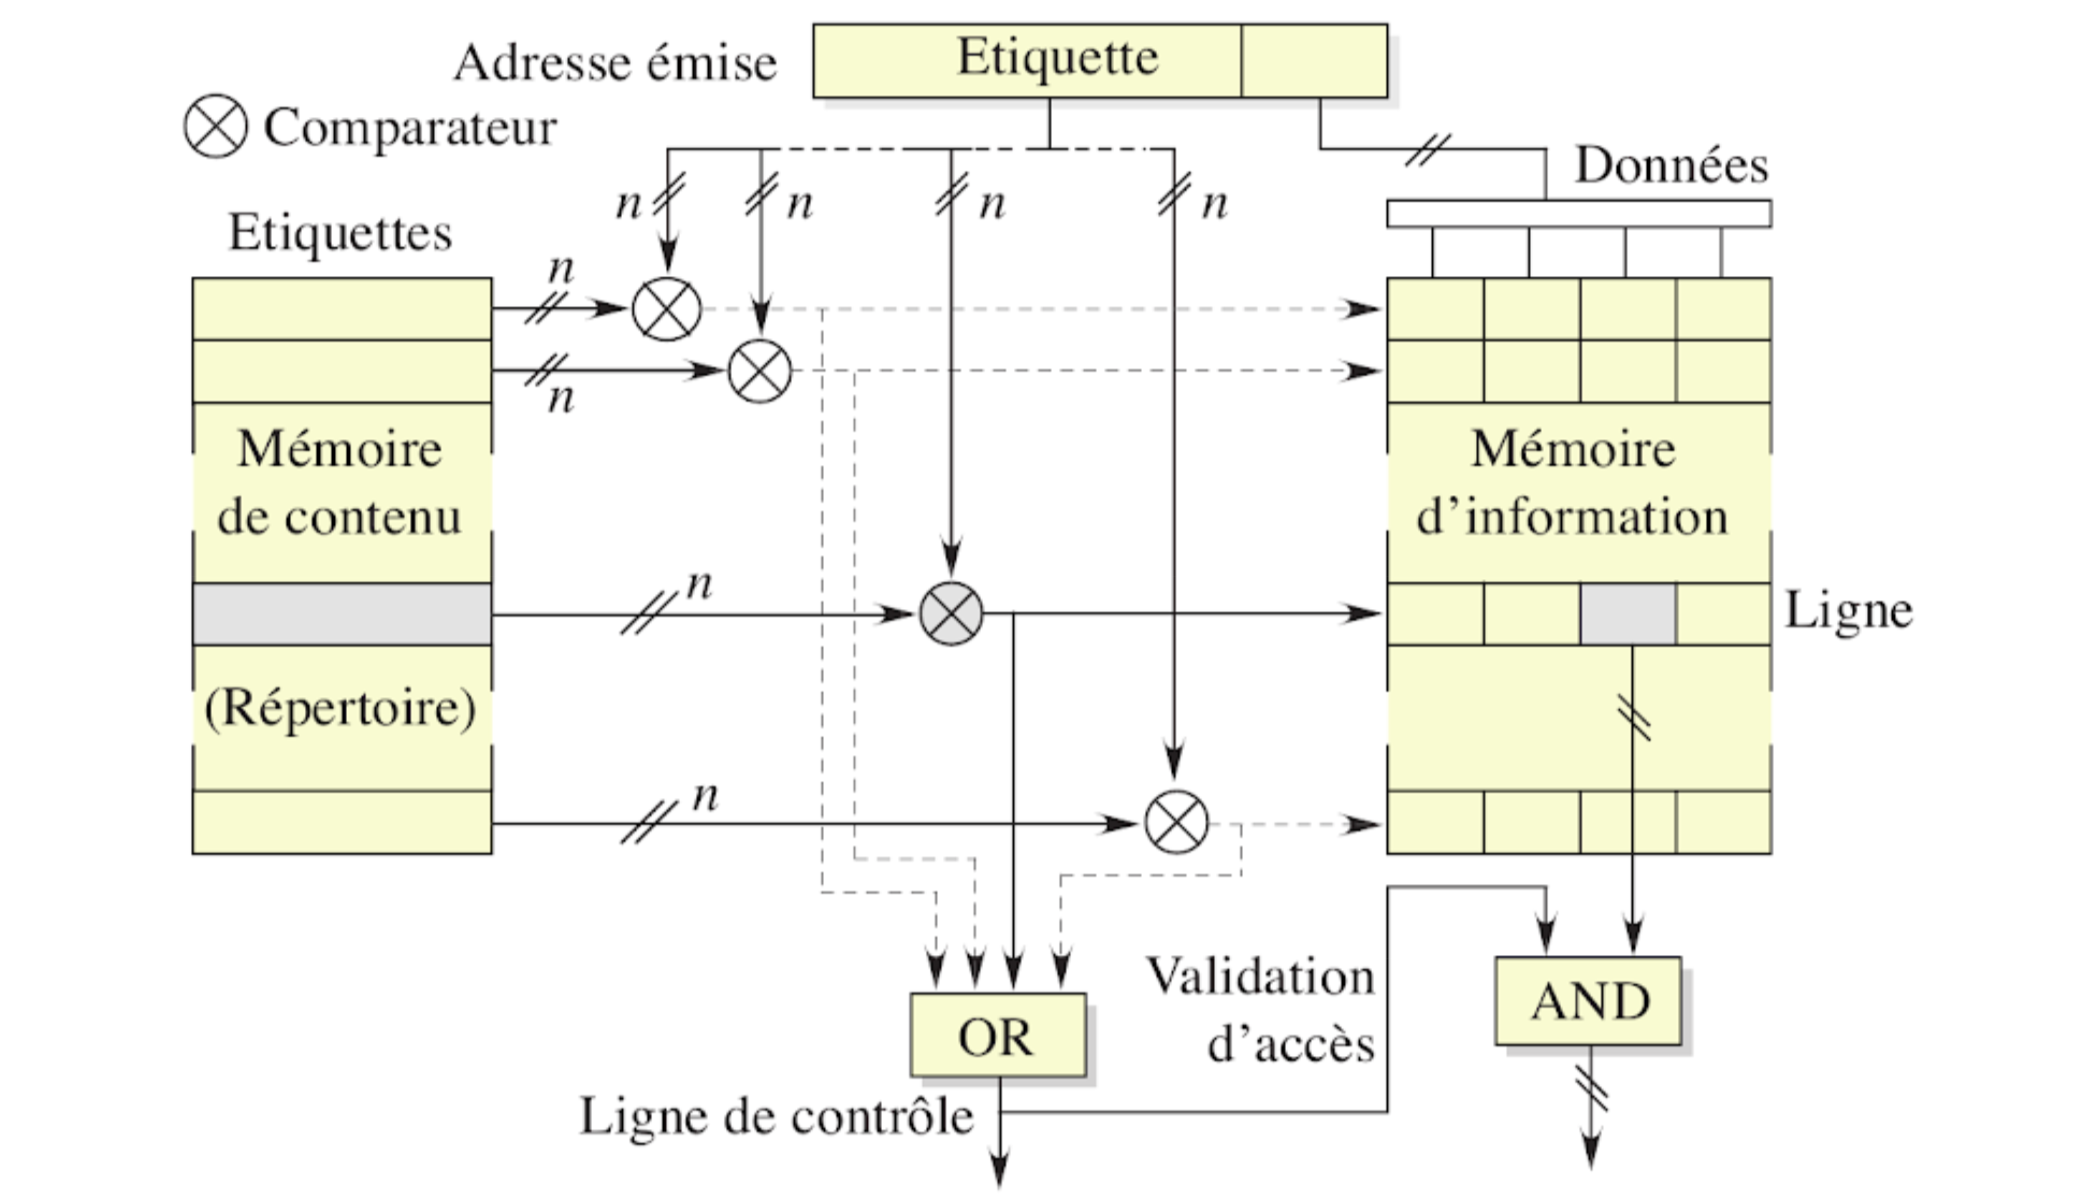
\includegraphics[width=\linewidth]{images/cache_circuit-fully-associative.png}
        \caption{Le cache pleinement associatif nécessite d'avoir un comparateur pour chacune des lignes du cache}
        \label{pic:cache_circuit-fully-associative}
    \end{subfigure}
    
    \begin{subfigure}[b]{0.45\linewidth}
        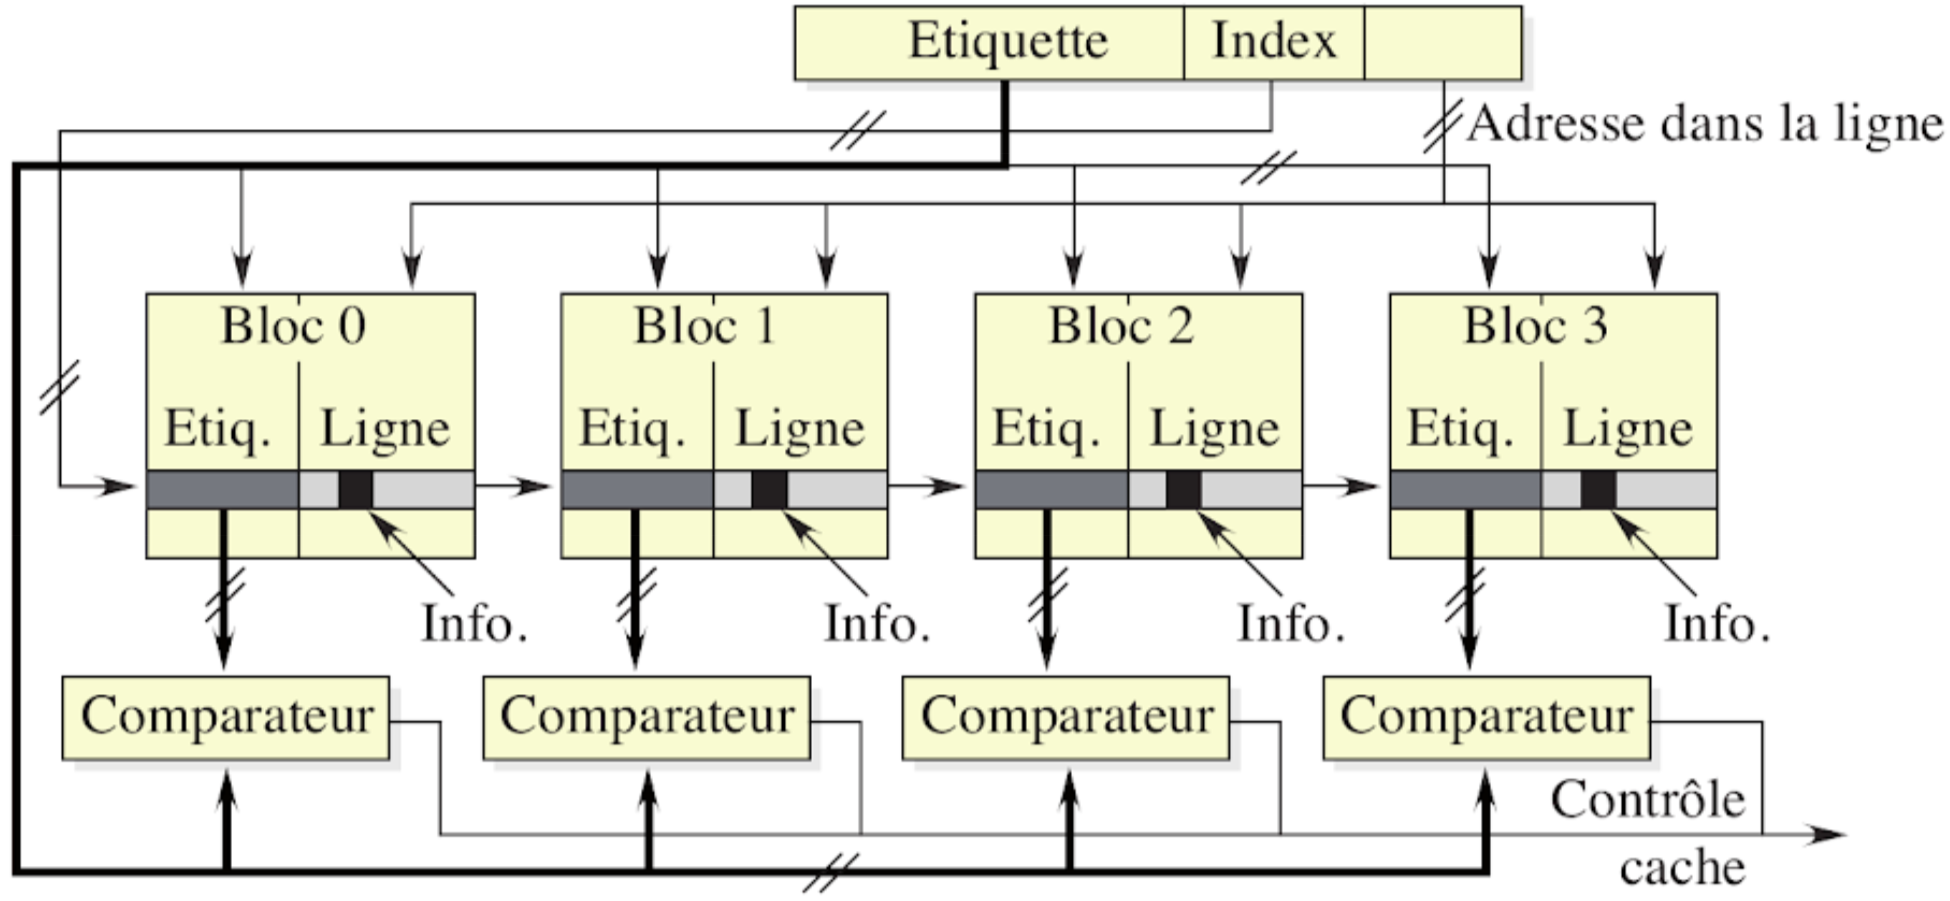
\includegraphics[width=\linewidth]{images/cache_circuit-set-associative.png}
        \caption{Le cache N-associatif associe les deux architectures des caches direct et pleinement associatif. Ce sont plusieurs caches directs montés en parallèles.}
        \label{pic:cache_circuit-set-associative}
    \end{subfigure}
    
    \caption{Schéma des trois modèles de cache utilisés (tirés de l'ouvrage \cite{Blanchet2013}).}\label{fig:cache_schema}
\end{figure}




\subsubsection{Politique de remplacement}
%%%%%%%%%%%%%%%%%%%%%%%%%%%%%%%%%%%%%%%%%%%%%%%%%%%%%%%%%%%%%%%%%%%
Que ce soit pour le mappage \textit{fully associative} ou \textit{set associative}, une \textit{cache line} peut être stockée dans plusieurs ligne du cache. Pour déterminer laquelle choisir pour y placer la \textit{cache line}, différentes stratégies peuvent être utilisées, appelées \textit{politique de remplacement}. L'objectif de ces politiques est de maximiser l'utilisation du cache en prévoyant et en anticipant les futures lignes à être accéder pour ne pas les supprimer du cache. Il existe de nombreuses politiques de remplacement, chacune ayant ses avantages et ses inconvénients \cite{wikipedia2_2019}: FIFO, LIFO, LRU, TLRU, MRU, PLRU, RR, SLRU, LFU, LFRU, LFUDA, LIRS, ARC, CAR, MQ. La politique choisie à un réelle impacte sur les performances de l'application. Pour la choisir, il faut trouver un compromis entre la performance la complexité apportée par la mise en place de la politique choisie. Dans le cas du mappage \textit{direct}, la ligne de cache présente à l'emplacement calculé est forcément remplacée et ne nécessite pas d'avoir une politique de remplacement. Il existe deux familles de politiques de remplacement. La première famille regroupe les politiques de remplacements qui tiennent compte de l'utilisation des \textit{cache line} (LRU, FIFO). Ce sont généralement les politiques les plus efficaces. La deuxième famille est celle des politiques aléatoires (\textit{random}, \textit{round robin}) qui ne tiennent pas compte de l'utilisation des données et choisissent une ligne aléatoirement à remplacer. Ces politiques sont performantes en termes de rapidité d'exécution car le choix ne se fait que sur une fonction aléatoire. Cependant, \cite{Al-Zoubi:2004:PEC:986537.986601} montrent que ces techniques utilisent 22\% moins bien le cache, impactant fortement les performances des applications.


\paragraph{Least Recently Used} ou LRU remplace la ligne de cache la moins récemment utilisée. Les numéros des lignes utilisée sont stockée dans une pile suivant la date de leur dernière utilisation. La pile est mise à jour lorsqu'une nouvelle donnée est stockée dans le cache en empilant son adresse au sommet de la pile. De même, lors d'un \textit{hit}, la ligne de cache référencé est stockée elle aussi en sommet de pile. Cette méthode à un inconvénient pour certains type d'accès, notamment les parcours de tableau. Imaginons un cache pouvant contenir 4 lignes. Le double parcours d'un tableau mesurant 5 ligne de caches a,b,c,d,e aura les accès mémoire suivant: a,b,c,d,e a,b,c,d,e. Le deuxième accès au tableau ne profitera pas du cache car chaque ligne de cache est remplacée au fur et mesure du parcours du tableau. Des améliorations ont été apportées pour corriger ce problème, comme l'introduction d'un répertoire image \cite{Stone:1987:HCA:31845} qui garde une trace des groupes de lignes de cache utilisées ensemble pour prévoir les accès similaires et anticiper leur accès.






\subsubsection{Stratégie de cache: lecture et écriture}
%%%%%%%%%%%%%%%%%%%%%%%%%%%%%%%%%%%%%%%%%%%%%%%%%%%%%%%%%%%%%%%%%%%

Le cache est une zone mémoire qui évolue en fonction des accès mémoires. Son fonctionnement lors d'un accès (en lecture ou écriture) peut varier en fonction de la présence (\textit{hit}) ou non (\textit{miss}) de la donnée et de la stratégie de cache implémentée.

\paragraph{Lecture:}  Lorsque le processeur accède à une donnée, il vérifie qu’elle n’est pas présente dans ses différents niveaux de cache. Si la donnée est présente, son accès est très rapide. Si ce n’est pas le cas, il réalise alors une copie de la zone mémoire la contenant dans le cache (la taille de la zone est une ligne de cache).

Lire en fonction des inclusion exclusion

\paragraph{Écriture:} la comportement du cache lors d'une écriture dépend de la présence ou non de la \textit{cache line} et la politique employée.

Si la ligne de cache n’est pas présente (\textit{miss}) dans le cache, deux solutions sont possibles. La première est de charger la ligne depuis la mémoire et d’y apporter les modifications (politique \textit{Write-Allocate}). La deuxième solution est d’écrire la ligne de cache sans la charger (politique \textit{No-Write-Allocate}). La ligne de cache ne sera chargé que lors d’un miss lors d’une lecture, sauf si la totalité de la ligne a été écrite, les données originales n'ayant plus de valeur utile. Cette option peut être intéressante si un algorithme ne fait qu’écrire dans un structure de donnée sans ne jamais la lire.

Si la ligne de cache est présente (\textit{hit}) dans le cache, deux solutions sont possibles. La première est de mettre à jour la \textit{cache line} dans le cache et en mémoire pour que le changement soit répercuter sur l'ensemble de la hiérarchie mémoire (politique \textit{Write-Through}). Cette politique peut être pénalisante si le processeur effectue consécutivement la mise à jour d'une donnée (par exemple un compteur, ou un index de bouble).  La seconde solution est de différer l'écriture à plus tard (politique \textit{Write-Back}). L’écriture est effectuée seulement dans le cache et ne sera effective en mémoire seulement lorsque la ligne de cache modifiée sera évincé du cache. La ligne de cache modifiée est alors indiqué grâce à un bit indicatif (\textit{dirty bit}). Comparé à la première méthode, celle ci utilise moins de bande passante car les mises à jour en mémoire sont moins fréquentes. Cependant, si plusieurs coeurs utilisent la même donnée, sa valeur pourrait alors être différente entre leurs caches respectifs (donnée périmée). Il faut alors implémenter un protocole de cohérence de cache entre les différents cache et la mémoire.

Les politiques utilisées lors d'un \textit{miss} ou d'un \textit{hit} peuvent être associés. Les combinaisons les plus utilisées sont \textit{Write-Through} + \textit{No-Write-Allocate} et \textit{Write-Back} + \textit{Write-Allocate}.






\subsubsection{Cohérence de cache} \label{sec:cache_coherence}
%%%%%%%%%%%%%%%%%%%%%%%%%%%%%%%%%%%%%%%%%%%%%%%%%%%%%%%%%%%%%%%%%%%

La stratégie employée lors de la modification d'une donnée introduit une challenge majeur des architectures multi-coeurs qui est de garantir la cohérence des données entres les différentes zones mémoires. Lors d'un accès mémoire, on souhaite accéder à la valeur sa plus récente, qui aura pû être modifiée par un autre coeur, ou processeur. La gestion de la cohérence d'un processeur à un seul coeur est plus simple, bien qu'elle doive tout de même être implémentée. Les opérations d'entrée-sortie peuvent affecter des données en mémoire qui se trouve aussi dans les caches.

Le protocole de cohérence de cache est responsable de vérifier qu'une même ligne de cache présente à plusieurs emplacement de la mémoire soit identique. Il doit pour cela garantir trois trois points. Le premier est de partager le changement d'une valeur à tous les coeurs d'un processeur pour que l'ordre des opérations affecté à une valeur soit vu dans le même ordre par tous les coeurs/processeurs. Le deuxième point est d'assurer que le résultat ne dépende que de l'ordre des instructions du programme assembleur et non de l'ordre de leur exécution par les différents coeurs. Enfin, le protocole doit assurer à un coeur qui lit une donnée que sa valeur est bien la dernière qui a été écrite (par un autre coeur ou autre processeur). La notion d'ancienneté peut être défini de plusieurs façons et le protocole doit la définir précisément pour assurer la validité des résultats \cite{Blanchet2013}. En effet, l'ordre peut faire référence à l'ordre des instructions dans le programme source. L'ordre peut aussi faire référence à celui de la fin des exécutions des résultats (avant que la donnée soit effectivement écrites). Enfin, ce peut être l'ordre des écritures mémoires. Comme la durée de propagation des écritures n'est pas constante dans le système, des erreurs peuvent apparaître si un protocole venait à utiliser ce dernier.

Comme le résume \cite{Blanchet2013}, les deux propriétés principales d'un protocole de cohérence sont sa simplicité de mise en oeuvre et sa performance. Pour assurer la cohérence, deux familles de protocoles existent, suivant si la gestion de cohérence est répartie sur les différents caches (\textit{locale}), ou si elle est centralisée (\textit{globale}). 



\paragraph{Protocoles locaux - cohérence répartie}

Les protocoles \textit{locaux} utilisent des outils de scrutation (\textit{snooping}) et de signalisation (\textit{broadcasting}). Implémentés directement dans les caches, ils ne nécessitent pas la modification ni de la mémoire ni du processeur. Lorsqu'une \textit{cache line} est modifié dans un cache, il obtient la copie exclusive de celle ci en invalidant ses copies dans d'autres caches (\textit{Write-Invalidate}). Une seconde option vise à simplement signaler la modification de cette ligne aux autres caches pour qu'ils mettent à jour leur structure de donnée (\textit{Write-Update}).  Différents protocoles de cohérence ont été implémentés et ont évolué. Les plus connues sont les protocoles MESI (ou \textit{Illinois}) \cite{papamarcos1984low} et MOESI. Mais il en existe beaucoup d'autres: MSI, MOSI, MERSI, MESIF. MESI et MOESI sont notamment très utilisés dans les processeurs multi-coeurs car il implémente des stratégies à écriture différée, minimisant le traffic mémoire.
\\
Nous présentons le protocole \textit{MOESI} à titre d'exemple. \textit{MOESI}  permet à une ligne de cache d'avoir cinq états différents. Le passage entre les différents état est résumé dans la \autoref{pic:moesi}. Chaque coeur surveille toutes les commandes effectuées sur le bus pour mettre à jour l'état de ses lignes ou les communiquer quand il en est propriétaire.

L'état $M$ (\textit{modified)} indique que la ligne est valide et qu'elle a été modifiée dans ce niveau de cache et qu'elle est seulement présente dans ce cache. La valeur en mémoire n'est pas cohérente, la ligne doit alors être copiée en mémoire lors de son remplacement. 

L'état $O$ (\textit{owned} ou \textit{shared-modified}) indique que cette ligne est valide est qu'elle est présente dans au moins un autre niveau de cache. Le cache actuel est \textit{propiétaire} de cette ligne, il doit informer les autres caches lors de sa modification. La ligne modifiée peut ensuite être communiqué à un autre niveau de cache, sans avoir à passer par la mémoire. Cet état est la principale amélioration apporté par le protocole \textit{MOESI} au protocole \textit{MESI}.


L'état $E$ (\textit{exclusive}) indique que la ligne est valide uniquement dans ce niveau de cache. Cela évite l'émission d'invalidation aux autres caches qui ne détiennent pas cette ligne. De plus, sur un autre cache y accède, la ligne de cache peut directement être transférée depuis le cache sans accès mémoire. La ligne dans le premier cache passera alors de l'état $E$ à $O$. Dans le deuxième cache la ligne sera en état $S$.

L'état $S$ (\textit{shared}) indique que la ligne est valide dans le cache courant et dans au moins un autre cache. Le cache actuel n'est pas propriétaire de la ligne (état $O$). La cohérence avec la mémoire n'est pas assumée. 

L'état $I$ (\textit{invalid}) indique que la ligne n'est pas valide. La lecture de cette ligne est interdite.


\begin{figure}
    \center
    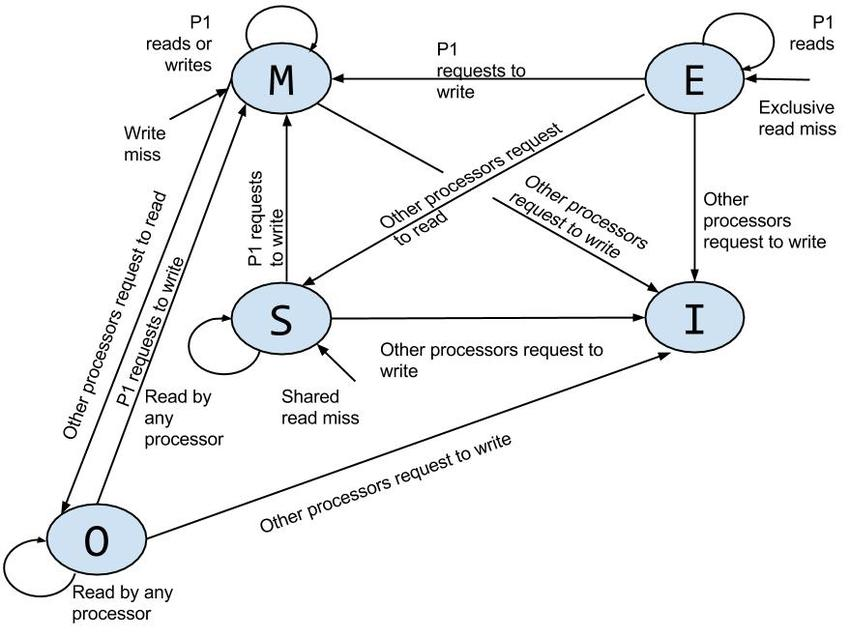
\includegraphics[width=10cm]{images/moesi.png}
    \caption{\label{pic:moesi} Fonctionnement du protocole MOESI (source \cite{Sayin2014})}
\end{figure}





\paragraph{Protocole globaux - Cohérence par répertoire (\textit{directory based coherence}}

La seconde famille regroupe les protocoles dits \textit{globaux} utilisent des répertoires et des controleurs émettant les commandes de transferts des lignes de cache (entre les caches ou avec la mémoire)\cite{tang1976cache}. Toutes les informations nécessaire à la gestion de la cohérence sont enregistrées dans un répertoire. Leur performance est meilleure que les protocoles utilisant des techniques de \textit{snooping} et \textit{broadcasting} car ils génèrent moins de trafic. Bien que les protocoles tel que MOESI réduise le trafic mémoire en utilisant des écritures différés, la gestion des cinq états est complexe. Et le trafic généré par la cohérence de cache augmente fortement avec le nombre de coeurs utilisés et peu rapidement voir ses performances s'effondrer \cite{liu2016protocoles}. Les futures architectures à mémoire partagée nécessiteront d'implémenter des protocole de cohérence de cache très performant  \cite{al2010snoopy}.


















%%%%%%%%%%%%%%%%%%%%%%%%%%%%%%%%%%%%%%%%%%%%%%%%%%%%%%%%%%%%%%%%%%%
%%%%%%%%%%%%%%%%%%%%%%%%%%%%%%%%%%%%%%%%%%%%%%%%%%%%%%%%%%%%%%%%%%%
\subsection{Mémoire principale}
%%%%%%%%%%%%%%%%%%%%%%%%%%%%%%%%%%%%%%%%%%%%%%%%%%%%%%%%%%%%%%%%%%%
%%%%%%%%%%%%%%%%%%%%%%%%%%%%%%%%%%%%%%%%%%%%%%%%%%%%%%%%%%%%%%%%%%%










